
\chapter{Podstawy teoretyczne}

% Rozdział teoretyczny --- przegląd literatury naświetlający stan wiedzy na dany temat. 
% TODO RL - opis oraz adaptacja w rozwiązaniu
% TODO Więcej badań trasowania płytek
% TODO Opis Badania i rejestracja przebiegu badania dla RL_PCB
% TODO Więcej wniosków dla Trasowania i wnioski dla placementu

W tej sekcji zawarte są definicje związane z problemem.

Przedmiotem badań jest zastosowanie sztucznej inteligencji w~dwóch etapach
projektowania PCB: rozmieszczaniu elementów (ang.~\emph{placement}) oraz
trasowaniu połączeń (ang.~\emph{routing}). Rozmieszczanie badane jest
z~użyciem metody uczenia ze wzmocnieniem (ang.~\emph{reinforcement learning},
RL) opracowanej przez L.~Vassallo i~J.~Bajadę~\cite{Vassallo2024RLPCB,Vassallo_RLPCB_GitHub},
a~trasowanie --- z~użyciem metody Unet-Astar opracowanej przez S.~Yina
i~współautorów~\cite{Yin2023UnetAstar,Firesuiry_UnetAstar_GitHub}.

\section{Budowa PCB}

Płytka drukowana (ang.~\emph{printed circuit board}, PCB) to produkt powstały
w wyniku selektywnego wytrawiania zbędnej miedzi z powierzchni izolacyjnych
podłoży pokrytych miedzią, tworzący wymaganą mozaikę połączeń, która jest
metalizowana i laminowana~\cite[pkt 3.2.53]{ECSS_Q_ST_70_12C_Rev1}.
Przekrój płytki dwuwarstwowej przedstawiono na rysunku~\ref{rys:przekroj-pcb}.
\emph{WARSTWA TOP} oraz \emph{WARSTWA BOTTOM} oznaczają międziane ścieżki.
Widać też przelotki, łączące górną i~dolną warstwę. Warstwy przedzielone
są materiałem izolującym, czyli laminatem oznaczonym na rysunku jako \emph{RDZEŃ}.

Na etapie projektowania płytkę można opisać dwoma modelami. Model logiczny
tworzą sieci, określające, które pady mają być ze sobą połączone. Model fizyczny
tworzą footprinty wraz z padami oraz ścieżki, przelotki i wypełnione obszary
miedzi~\cite{KiCad_PCBEditor_BasicConcepts}.

Płytki jedno- i dwustronne są najczęściej wykorzystywane w urządzeniach
codziennego użytku~\cite{Romik_TSPCB_ObwodDrukowany} i to one będą przedmiotem
badań. Liczba warstw miedzi jest ograniczona także przez oprogramowanie
projektowe; KiCad obsługuje ich do~32~\cite{KiCad_PCBEditor_BasicConcepts}.

\begin{figure}[H]
\centering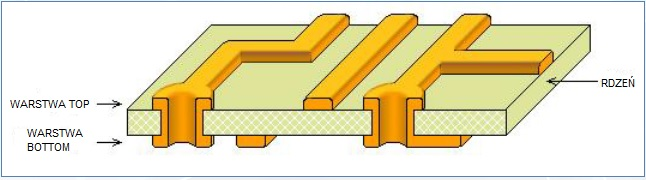
\includegraphics[width=\textwidth]{figures/Bez-tytulu}
\caption{Przekrój płytki PCB. Źródło:~\cite{Romik_TSPCB_ObwodDrukowany}.}\label{rys:przekroj-pcb}
\end{figure}

\subsection{Elementy PCB}

\begin{description}
  \item[Warstwa przewodząca] (ang.~\emph{conductive layer}) --- elementy
    przewodzące płytki leżące na tej samej warstwie, np.~ścieżki, płaszczyzny
    lub pady~\cite[pkt 3.2.18]{ECSS_Q_ST_70_12C_Rev1}.
  \item[Footprint] --- reprezentacja elementu elektronicznego na płytce wraz
    z jego padami~\cite{KiCad_PCBEditor_BasicConcepts}.
  \item[Pad] (pole lutownicze, ang.~\emph{soldering pad}) --- element
    przewodzący przeznaczony do przylutowania komponentu do
    płytki~\cite[pkt 3.2.62]{ECSS_Q_ST_70_12C_Rev1}.
  \item[Sieć] (ang.~\emph{net}) --- określenie, w jaki sposób pady mają być ze
    sobą połączone~\cite{KiCad_PCBEditor_BasicConcepts}.
  \item[Ścieżka] (ang.~\emph{track}) --- element przewodzący prowadzący
    połączenie elektryczne między padami~\cite[pkt 3.2.66]{ECSS_Q_ST_70_12C_Rev1}.
  \item[Przelotka] (ang.~\emph{via}) --- metalizowany otwór służący wyłącznie
    do łączenia warstw~\cite[pkt 3.2.67]{ECSS_Q_ST_70_12C_Rev1}.
  \item[Wypełniony obszar miedzi] (ang.~\emph{filled zone}) --- obszar miedzi
    tworzący, obok ścieżek i przelotek, połączenia między padami danej
    sieci~\cite{KiCad_PCBEditor_BasicConcepts}.
\end{description}

\section{Problem placementu}
\label{sec:problem-placementu}

% TODO: definicja problemu rozmieszczania elementów (dane wejściowe, wynik,
% ograniczenia, kryteria oceny -- analogicznie do sekcji o routingu).

\section{Problem routingu}

w problemie routingu, sieci są danymi wejściowymi a na wyjściu oczekuje się modelu fizycznego płytki. Jednak w praktyce
rozmieszczenie elementów na płytce jest z góry narzucone a zatem również można traktować je jako daną wejściową - co spłyca
problem routingu do samego prowadzenia ścieżek i rozmieszczania przelotek.

\begin{description}
  \item[Dane wejściowe] --- obrys płytki, liczba warstw, rozmieszczone
    footprinty, sieci oraz reguły projektowe.
  \item[Wynik] --- ścieżki i przelotki łączące pady każdej sieci.
  \item[Ograniczenia] --- brak zwarć między różnymi sieciami, zachowanie
    minimalnych odstępów i szerokości ścieżek.
  \item[Kryteria oceny] --- odsetek połączonych sieci, łączna długość ścieżek,
    liczba przelotek.
\end{description}

\section{Reguły projektowe}

Programy do projektowania płytek takie jak EasyEDA lub KiCad posiadają wbudowane narzędzie do weryfikacji,
czy określone wymagania dotyczące płytki zostały spełnione oraz czy wszystkie pady zostały połączone zgodnie z
netlistami. Narzędzie to nosi nazwę DRC (ang. Design Rule Checker). W przypadku KiCada narzędzie automatycznie
zapobiega łamaniu niektórych reguł podczas trasowania ścieżek. Nadal jednak istnieje wiele regół których w ten
sposób nie da się wykluczyć, gotowy schemat oraz przygotowaną płytkę należy zatem walidować.~\cite{KiCad_PCBEditor_DRC}:

\begin{description}
  \item[Minimalny odstęp izolacyjny] (ang.~\emph{clearance}) --- najmniejsza
    dopuszczalna odległość między elementami miedzi należącymi do różnych sieci.
  \item[Szerokość ścieżki] (ang.~\emph{track width}) --- minimalna, zalecana
    i~maksymalna szerokość ścieżki. Wraz z~odstępem izolacyjnym decyduje, ile
    ścieżek można poprowadzić między sąsiednimi padami.
  \item[Wymiary przelotki] --- średnica przelotki, średnica otworu oraz
    szerokość pierścienia miedzi wokół otworu (ang.~\emph{annular width}).
    Przelotka zajmuje miejsce na każdej warstwie, przez którą przechodzi.
  \item[Odstęp od krawędzi płytki] (ang.~\emph{edge clearance}) --- minimalna
    odległość miedzi od obrysu płytki, wynikająca z~tolerancji frezowania.
  \item[Odstęp obrysów elementów] (ang.~\emph{courtyard clearance}) ---
    minimalna odległość między obrysami zajmowanymi przez footprinty; ich
    nachodzenie na siebie jest błędem.
  \item[Obszary zabronione] (ang.~\emph{keepout}) --- obszary, w~których nie
    wolno umieszczać wskazanych obiektów, np.~ścieżek, przelotek lub footprintów.
  \item[Ograniczenia integralności sygnału] --- dopuszczalna długość połączenia
    (ang.~\emph{length}), różnica długości połączeń (ang.~\emph{skew}) oraz
    odstęp między ścieżkami pary różnicowej (ang.~\emph{differential pair gap}).
\end{description}

Za poprawne rozwiązanie problemu routingu można uznać takie, w~którym DRC nie
wykazuje zwarć między sieciami (\emph{Items shorting two nets}), naruszeń
odstępów (\emph{Clearance violation}) ani niepołączonych elementów sieci
(\emph{Missing connection between items})~\cite{KiCad_PCBEditor_DRC}.

Rozwiązania oparte na sztucznej inteligencji uwzględniają reguły projektowe
w~uproszczonej postaci. Zestawienie dla dwóch rozwiązań z~otwartym kodem
przedstawiono w~tabeli~\ref{tab:reguly-ai}.

\begin{table}[ht]
\fcmtcaption{Uwzględnienie reguł projektowych w~rozwiązaniach Unet-Astar
i~RL\_PCB. Źródło: opracowanie własne na podstawie kodu
źródłowego~\cite{Firesuiry_UnetAstar_GitHub,Vassallo_RLPCB_GitHub}.}\label{tab:reguly-ai}
\centering\footnotesize%
\begin{tabular}{p{0.22\textwidth} p{0.34\textwidth} p{0.34\textwidth}}
\toprule
Reguła & Unet-Astar (trasowanie) & RL\_PCB (rozmieszczanie) \\
\midrule
Odstęp izolacyjny & jedna wartość dla całej płytki, zaokrąglana w~górę do
  siatki & nie dotyczy \\
  \midrule
Szerokość ścieżki & jedna wartość dla całej płytki & nie dotyczy \\
\midrule
Klasy sieci & nieobsługiwane & nie dotyczy \\
\midrule
Wymiary przelotki & jeden rozmiar (najmniejszy z~pliku wejściowego) & nie
  dotyczy \\
  \midrule
Odstęp obrysów elementów & nie dotyczy (rozmieszczenie jest daną wejściową)
  & ograniczenie miękkie: kara w~funkcji nagrody; w~ocenie dopuszczano do
  20\% nakładania \\
  \midrule
Obrys elementu & nie dotyczy & prostokąt o~wymiarach elementu \\
\midrule
Orientacja elementu & nie dotyczy & obroty o~wielokrotność $90^\circ$ \\
\midrule
Trasowanie w~ocenie & --- & zewnętrzny program, z~pominięciem sieci zasilania \\
\bottomrule
\end{tabular}
\end{table}

% TODO ogólny opis algorytmów a nie zastosowanie ich w programach

\section{Algorytm A*}
A* jest heurystycznym algorytmem służącym do znajdowanias najkrótszej ścieżki w grafie.
Jest to algorytm zupełny i optymalny, a zatem zawsze da się znaleźć przy jego pomocy
najlepsze rozwiązanie. Metoda gwarantuje, że każdy punkt zostanie odwiedzony dzięki zorganizowanemu
modelowi pamięciowemu.

Działanie oparte jest na minimalizacji funkcji celu $f(x)$, zdefiniowanej jako suma funkcjo kosztu
$g(x)$ oraz funkcji heurystycznej $h(x)$:
\begin{equation}
  f(x) = g(x) + h(x)
  \label{eq:astar-f}
\end{equation}

W każdym krokui A* przedłuża już utworzoną ścieżkę o kolejny wierzchołek grafu wybierając taki,
w którym wartość funkcji $f$ będzie najmniejsza.

Funkcja $g(x)$ określa rzeczywisty koszt dojścia do punktu $x$ (suma wag krawędzi należących do ścieżki
oraz wagi krawędzi łączącej aktualny węzeł z $x$).

funkcja $h(x)$ funkcja heurystyczna. Oszacowuje w sposób optymistyczny koszt dotarcia od punktu $x$
do wierzchołka docelowego.

warunki prawidłowości funkcji heurystycznej:

warunek dopuszczalności
\begin{equation}
  g(x) + h(x) \le g(x_t),
  \label{eq:astar-dopuszczalnosc}
\end{equation}
gdzie $x_t$ oznacza punkt końcowy.

warunek monotoniczności
\begin{equation}
  g(x_j) + h(x_j) \ge g(x_i) + h(x_i),
  \label{eq:astar-monotonicznosc}
\end{equation}
gdzie $j > i$.

\subsection{Adaptacja algorytmu A* w~metodzie Unet-Astar}
\label{sec:astar-unet}

Algorytm trasowania w~metodzie Unet-Astar opiera się na algorytmie A*
zaproponowanym przez T.-C.~Lina i~in.\ do ujednoliconego trasowania płytek
PCB~\cite{Lin2021UnifiedPCB,Yin2023UnetAstar}. Płytkę przedstawia się jako
trójwymiarową siatkę, w~której węzeł odpowiada oczku siatki na danej
warstwie miedzi. Ścieżka jest drogą w~tym grafie między węzłami
odpowiadającymi dwóm padom, a~przejście między warstwami odpowiada
przelotce.

W~odróżnieniu od algorytmu bazowego Unet-Astar stosuje zmodyfikowaną funkcję
oceny węzła~\cite{Yin2023UnetAstar}:
\begin{equation}
  f(c) = g(s, c) + h(c, t) - P_{\mathrm{lin}} \cdot r(c),
  \label{eq:unet-astar-koszt}
\end{equation}
gdzie $g(s,c)$ oznacza koszt dojścia od punktu początkowego $s$ do bieżącego
węzła $c$, a~$h(c,t)$ oszacowanie kosztu dojścia od węzła $c$ do punktu
docelowego $t$. Koszt obejmuje długość ścieżki, karę za załamania
oraz karę za naruszenie reguł projektowych. Wartość $r(c) \in [0,1]$ to
wartość obszaru rekomendowanego w~węźle $c$, przewidziana przez sieć
neuronową przed rozpoczęciem trasowania połączenia. Hiperparametr
$P_{\mathrm{lin}}$ (ang.~\emph{liner-power}) określa kompromis między
podążaniem za obszarem rekomendowanym a~kosztem trasowania. Im większa jego
wartość, tym silniej algorytm preferuje węzły wskazane przez sieć i~tym
mniej węzłów spoza obszaru rekomendowanego rozwija. Odjęcie składnika
zależnego od $r(c)$ sprawia, że heurystyka przestaje być dopuszczalna
w~sensie warunku~(\ref{eq:astar-dopuszczalnosc}). Algorytm nie gwarantuje
więc już ścieżki o~najmniejszym koszcie, ale w~zamian przeszukuje znacznie
mniejszą część siatki.

Wiele krótkich połączeń na płytce jest na tyle prostych, że obszar
rekomendowany niewiele przyspiesza ich poprowadzenie. Dlatego wprowadzono
drugi hiperparametr, $p_{\mathrm{skip}}$ (ang.~\emph{skip-percent}).
Połączenia szereguje się według długości. Następnie najkrótsze połączenia
stanowiące \emph{skip-percent} wszystkich połączeń prowadzi się
klasycznym algorytmem A*, bez użycia sieci~\cite{Yin2023UnetAstar}.
Analogicznie połączenia te pomija się przy tworzeniu próbek
uczących.

Trasowanie całej płytki przebiega w~następujących krokach~\cite{Yin2023UnetAstar}:
\begin{enumerate}
  \item Sieci wielopinowe dzieli się na połączenia dwupinowe za pomocą
    algorytmu drzewa Steinera.
  \item Połączenia dwupinowe szereguje się według długości odcinka łączącego
    ich końce, od najkrótszego do najdłuższego.
  \item Połączenia prowadzi się kolejno, zgodnie z~ustaloną kolejnością.
\end{enumerate}
Połączenia prowadzone są sekwencyjnie, więc każda poprowadzona ścieżka staje
się przeszkodą dla kolejnych. Na dużych i~gęstych płytkach algorytm A*
musi wtedy rozwinąć bardzo wiele węzłów, zanim znajdzie drogę omijającą
wcześniej poprowadzone ścieżki. Ograniczenie przeszukiwanego obszaru za
pomocą predykcji sieci neuronowej jest odpowiedzią właśnie na ten
problem.

\section{Algorytm Lee}
\label{sec:lee}

Algorytm Lee, zaproponowany przez C.~Y.~Lee w~1961~roku, służy do
wyznaczania połączenia między dwoma punktami na siatce z~przeszkodami.
Został opracowany z~myślą o~prowadzeniu połączeń w~układach
elektronicznych i~jest jednym z~pierwszych algorytmów trasowania płytek
drukowanych~\cite{Lee1961}. Płytkę przedstawia się jako siatkę oczek,
z~których każde jest wolne albo zajęte przez przeszkodę. Algorytm działa
w~dwóch fazach:
\begin{enumerate}
  \item \emph{Propagacja fali} --- oczko początkowe otrzymuje etykietę~0.
    Następnie wszystkie wolne, nieoznaczone sąsiednie oczka oczek
    z~etykietą $k$ otrzymują etykietę $k+1$. Fala rozchodzi się w~ten sposób
    równomiernie we wszystkich kierunkach, aż dotrze do oczka docelowego
    albo nie będzie już oczek do oznaczenia.
  \item \emph{Odtworzenie ścieżki} --- począwszy od oczka docelowego
    przechodzi się do dowolnego sąsiada o~etykiecie mniejszej o~1, aż do
    oczka początkowego. Uzyskany ciąg oczek jest najkrótszą ścieżką.
\end{enumerate}

Algorytm zawsze znajduje najkrótszą ścieżkę, jeżeli taka istnieje, ale
w~najgorszym przypadku oznacza wszystkie oczka siatki. Czas działania
i~zapotrzebowanie na pamięć rosną więc proporcjonalnie do powierzchni płytki:
dla siatki o~wymiarach $M \times N$ oczek wynoszą $O(MN)$~\cite{Zhou_EECS357_Lee}.
W~odróżnieniu od algorytmu A* propagacja nie jest kierowana heurystyką
w~stronę celu, dlatego algorytm odwiedza znacznie więcej oczek.

W~metodzie Unet-Astar dwukierunkowy wariant algorytmu Lee służy do
przygotowania danych uczących~\cite{Yin2023UnetAstar}. Fale propagowane są
jednocześnie z~punktu początkowego $s$ i~końcowego $t$, dzięki czemu dla
każdego oczka $n$ znane są odległości $d_s(n)$ i~$d_t(n)$ od obu końców
połączenia. Obszar rekomendowany tworzą oczka, przez które przechodzi
ścieżka niewiele dłuższa od najkrótszej:
\begin{equation}
  R = \{\, n : d_s(n) + d_t(n) \le L^* + 0{,}1 \cdot d(s, t) \,\},
  \label{eq:lee-obszar}
\end{equation}
gdzie $L^*$ oznacza długość najkrótszej ścieżki, a~$d(s,t)$ odległość
euklidesową między końcami połączenia~\cite{Yin2023UnetAstar}. Tak
wyznaczone obszary stanowią etykiety, na których uczona jest sieć
neuronowa. Podczas trasowania algorytm Lee nie jest już wykonywany ---
obszar rekomendowany przewiduje wytrenowana sieć.

\section{Konwolucyjne sieci neuronowe}

Konwolucyjne sieci neuronowe (ang.~\emph{convolutional neural networks}, CNN)
są zbudowane, podobnie jak klasyczne sieci neuronowe, z~neuronów, które
uczą się przez optymalizację swoich wag. Każdy neuron otrzymuje sygnały
wejściowe i~wykonuje na nich operację, np.~iloczyn skalarny, po którym
następuje nieliniowa funkcja aktywacji. Sieci te są stosowane przede
wszystkim do rozpoznawania wzorców w~obrazach, a~ich architektura
uwzględnia cechy tego rodzaju danych~\cite{OShea2015CNN}.

W~klasycznej sieci każdy neuron pierwszej warstwy ukrytej jest połączony
ze wszystkimi wartościami wejściowymi. Dla kolorowego obrazu o~wymiarach
$64 \times 64$ oznacza to $64 \cdot 64 \cdot 3 = 12\,288$ wag w~jednym
neuronie. Tak duża liczba parametrów wymaga dużej mocy obliczeniowej
i~zwiększa ryzyko przeuczenia (ang.~\emph{overfitting}), czyli utraty
zdolności uogólniania na dane spoza zbioru uczącego~\cite{OShea2015CNN}.

W~sieci konwolucyjnej neurony są uporządkowane w~trzech wymiarach:
wysokości, szerokości i~głębokości. Głębokość oznacza tu trzeci wymiar
danych, np.~liczbę kanałów obrazu, a~nie liczbę warstw sieci. Każdy neuron
jest połączony tylko z~niewielkim obszarem poprzedniej warstwy. Sieć
składa się z~trzech rodzajów warstw: konwolucyjnych, łączących
(ang.~\emph{pooling}) i~w~pełni połączonych~\cite{OShea2015CNN}.


\section{U-net}
- Rodzaj sieci konwolucyjnej, w skrócie: konwolucja, pooling, segmentacja obrazu 
(klasyfikacja każdego pixela).
- Część kodująca zmiejsza obraz i zbiera kontekst, a część dekodująca odtwarza rozdzielczość.
- Połączenia pomijające (skip connections) przekazują szczegóły przestrzenne z kodera do dekodera.

\section{Deeper U-Net i Unet-Astar}
- Pomysł z Artykułu: sieć wskazuje obszary rekomendowane, a głębsza struktura daje więcej informacji kontekstowej.
- Architektura w kodzie: wejście $256 \times 256$ z 3 kanałami, 8 redukcji rozdzielczości aż do $1 \times 1$, warstwa w pełni połączona
w środku i 2 klasy na wyjściu. Klasyczny U-Net ma 4 redukcje.
- Połączenie z A*: sieć nie zastępuje A*, tylko zmienia kolejność odwiedzania węzłów

\begin{equation}
  f'(n) = \bigl(f(n) - a \cdot s(n)\bigr) \cdot \bigl(1 - b \cdot s(n)\bigr),
  \label{eq:unet-astar-f}
\end{equation}
gdzie $s(n)$ to wynik sieci dla węzła, a domyślnie $a = b = 3$.
Dla $b = 0$ wzór sprowadza się do funkcji~(\ref{eq:unet-astar-koszt})
z~artykułu, przy $a = P_{\mathrm{lin}}$.

\section{Reinforcement Learning}

%TODO opis ogólny RL oraz adaptacja architektury sieci w RL PCB